\documentclass[tikz, border=3mm]{standalone}
\usepackage{tikz}
\usetikzlibrary{decorations.pathmorphing} % For random steps/snake decoration if needed
\usetikzlibrary{positioning} % For label positioning

\begin{document}
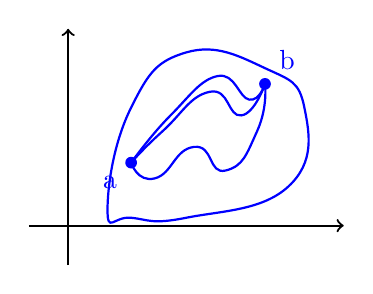
\begin{tikzpicture}[
    blob/.style={blue, thick}, % Style for the blob lines
    point/.style={fill=blue, circle, inner sep=1.5pt} % Style for points a and b
]

% Axes
\draw[->, thick] (-0.5, 0) -- (3.5, 0); % x-axis
\draw[->, thick] (0, -0.5) -- (0, 2.5); % y-axis

% Outer Blob - using plot smooth cycle for approximation
\draw[blob] plot [smooth cycle, tension=0.8] coordinates {
    (0.5, 0.2) (0.8, 1.5) (1.5, 2.2) (2.5, 2.0) (3.0, 1.5) (2.8, 0.5) (1.5, 0.1) (0.8, 0.1)
};

% Define coordinates for points a and b explicitly
\coordinate (a) at (0.8, 0.8);
\coordinate (b) at (2.5, 1.8);

% --- Inner Paths ---

% Path 1 (Original)
\draw[blob] plot [smooth, tension=0.9] coordinates {
    (a) (1.2, 1.2) (1.8, 1.7) (2.2, 1.4) (b)
};

% Path 2 (Slightly higher)
\draw[blob] plot [smooth, tension=0.8] coordinates {
    (a) (1.3, 1.4) (1.9, 1.9) (2.3, 1.6) (b)
};

% Path 3 (Slightly lower, more wiggly)
\draw[blob] plot [smooth, tension=1.0] coordinates {
    (a) (1.1, 0.6) (1.6, 1.0) (2.0, 0.7) (2.4, 1.2) (b)
};

% --- End Inner Paths ---


% Mark and Label Points a and b (Draw last to be on top)
\node[point, label={[blue]below left:a}] at (a) {};
\node[point, label={[blue]above right:b}] at (b) {};


\end{tikzpicture}
\end{document}